\chapter{Сучасний стан задачі побудови безхмарних супутникових знімків}
Отримання безхмарних супутникових знімків грає ключову роль в аналізі та моніторингу Землі. Тому так важливо мати якісні та оброблені знімки, щоб проводити власне дослідження. Тому для того, щоб розуміти навіщо потрібно розвивати дану технологію потрібно проаналізувати, що саме вона представляє на даний час.

На сьогодні одними із відомих компаній супутникового моніторингу Землі, що володіють своїми аналогами алгоритму вилучення хмар із супутникових знімків є американська Descartes Labs та австралійська EOxCloudless. Тому є необхідність зробити огляд їхніх безхмарних карт на предмет виявлення недоліків на знімках.

\section{Descartes Labs}
Descartes Labs використовує свої власне Python APIs.

Для побудови безхмарних зображень компанія застосовує дані супутників Landsat 8, Sentinel-1 SAR, Sentinel-2 Red Edge та аерозйомку, що покриває лише територію США.

При первинному аналізі карт даної організації, було виявлено дефектні полоси (Рисунок 1. 2), тобто різниця значень пікселів після склеювання.Як ми бачимо, на знімках в деяких регіонах присутньо багато хмарних пікселів (Рисунок 1. 1) та видно візуально різницю в пікселях після склейки знімків.

Таким чином можна сказати, що алгоритм отримання безхмарних знімків супутникових знімків від американської компанії Descartes Labs є не дуже якісним.

\begin{figure}[H]\centering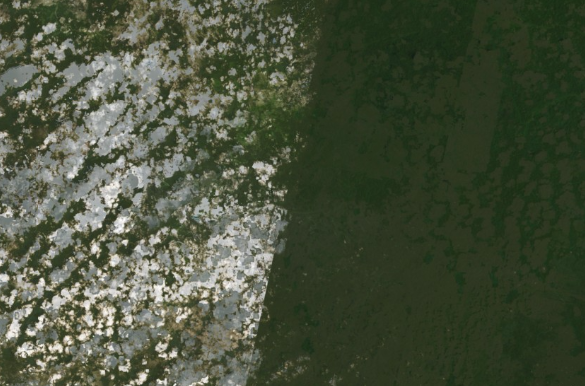
\includegraphics[width=0.82\textwidth]{images/image1.png}\caption{Ілюстрація з вихідної роботи (image1)}\label{fig:image1}\end{figure}
\begin{figure}[H]\centering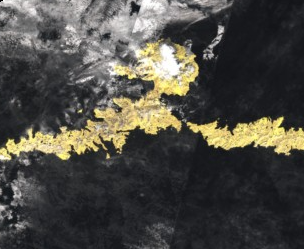
\includegraphics[width=0.82\textwidth]{images/image2.png}\caption{Ілюстрація з вихідної роботи (image2)}\label{fig:image2}\end{figure}
\section{EOxCloudless}
Іншою компанією , що спеціалізується на обробці супутникових даних є EOxCloudless. Вона аналізує дані із родини супутників Sentinel 1 та Sentinel 2. EOxCloudless забезпечує безперервний моніторинг сільськогосподарських просторових областей за допомогою оптичних даних більш високого рівня або навіть комбінації оптичних і радіолокаційних даних разом з оптимізованими інтервалами часу.

\begin{figure}[H]\centering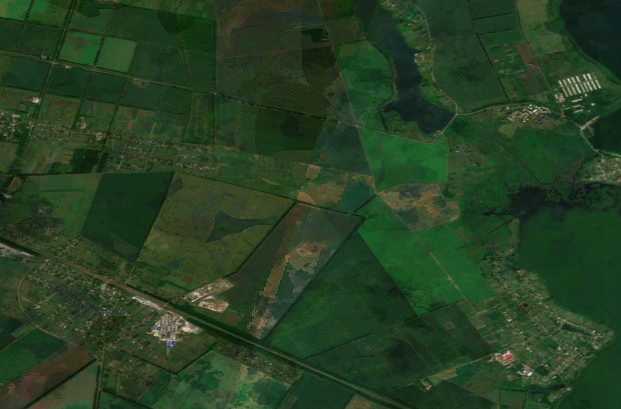
\includegraphics[width=0.82\textwidth]{images/image3.png}\caption{Ілюстрація з вихідної роботи (image3)}\label{fig:image3}\end{figure}
\begin{figure}[H]\centering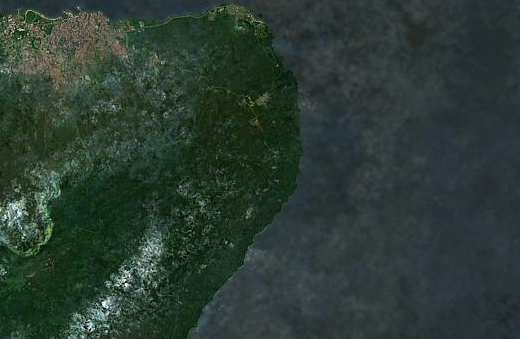
\includegraphics[width=0.82\textwidth]{images/image4.png}\caption{Ілюстрація з вихідної роботи (image4)}\label{fig:image4}\end{figure}
Отже, на знімках \cite{ref14} теж присутні дефекти (Рисунок 1. 4) хоч і не в такій кільості як на супутникових знімках попередньої компанії. В цьому випадку видно, колірна різниця між регіонами (Рисунок 1. 3), помітно менша і візуально картинка виглядає набагато краще.

На основі первинного аналізу результатів аналогів алгоритмів від компаній EOxCloudless , Descartes Labs, , було виявлене в деяких регіонах неякісні знімки та таке ж погане відновлення неповних даних.

Україні зараз необхідно мати свою безхмарну карту, оскільки це дозволить проводити ще якісніше моніторинг посівних площ чи аналіз культур, або ж застосовуватись водоканальними службами для відслідковування розливів водойм чи річок.

У дипломній роботі описані можливе вирішення проблеми неповних даних та зроблену власну модель, що дає безхмарний супутниковий знімок на основі знімків від сімейства супутників Sentinel 2. Хоча слід зазначити, що модель буде працювати на будь-яких 3 -канальних RGB супутникових даних.

\chapterConclusion
Було досліджено та проаналізовано сучасний стан побудови безхмарних супутникових знімків. Розглянуто приклади знімків, які дають компанії EoxCloudless та Descartes Labs, що володіють власними аналогами технології вилучення хмарних пікселів зі знімків. Виявлено їхні недоліки, та визначена потреба мати безхмарні супутникові зображення України.

